%%%%%%%%%%%%%%%%%%%%%%%%%%%%%%%%%%%%%%%%%%%%%%%%%%%%%%%%%%%%%%%%%%%%%
%% This is a (brief) model paper using the achemso class
%% The document class accepts keyval options, which should include
%% the target journal and optionally the manuscript type. 
%%%%%%%%%%%%%%%%%%%%%%%%%%%%%%%%%%%%%%%%%%%%%%%%%%%%%%%%%%%%%%%%%%%%%
\documentclass[journal=jacsat,manuscript=article]{achemso}

%%%%%%%%%%%%%%%%%%%%%%%%%%%%%%%%%%%%%%%%%%%%%%%%%%%%%%%%%%%%%%%%%%%%%
%% Place any additional packages needed here.  Only include packages
%% which are essential, to avoid problems later. Do NOT use any
%% packages which require e-TeX (for example etoolbox): the e-TeX
%% extensions are not currently available on the ACS conversion
%% servers.
%%%%%%%%%%%%%%%%%%%%%%%%%%%%%%%%%%%%%%%%%%%%%%%%%%%%%%%%%%%%%%%%%%%%%
\usepackage[version=3]{mhchem} % Formula subscripts using \ce{}

%%%%%%%%%%%%%%%%%%%%%%%%%%%%%%%%%%%%%%%%%%%%%%%%%%%%%%%%%%%%%%%%%%%%%
%% If issues arise when submitting your manuscript, you may want to
%% un-comment the next line.  This provides information on the
%% version of every file you have used.
%%%%%%%%%%%%%%%%%%%%%%%%%%%%%%%%%%%%%%%%%%%%%%%%%%%%%%%%%%%%%%%%%%%%%
%%\listfiles

%%%%%%%%%%%%%%%%%%%%%%%%%%%%%%%%%%%%%%%%%%%%%%%%%%%%%%%%%%%%%%%%%%%%%
%% Place any additional macros here.  Please use \newcommand* where
%% possible, and avoid layout-changing macros (which are not used
%% when typesetting).
%%%%%%%%%%%%%%%%%%%%%%%%%%%%%%%%%%%%%%%%%%%%%%%%%%%%%%%%%%%%%%%%%%%%%
\newcommand*\mycommand[1]{\texttt{\emph{#1}}}

\author{Valentin Zulkower}
\affiliation[University of Edinburgh]
{Edinburgh Genome Foundry, SynthSys Center for Synthetic and Systems Biology, School of Biological Sciences, University of Edinburgh, EH9 3BF Edinburgh, UK}
\email{valentin.zulkower@ed.ac.uk}
\author{Susan Rosser}
\affiliation[University of Edinburgh]
{Edinburgh Genome Foundry, SynthSys Center for Synthetic and Systems Biology, School of Biological Sciences, University of Edinburgh, EH9 3BF Edinburgh, UK}
\email{susan.rosser@ed.ac.uk}

%%%%%%%%%%%%%%%%%%%%%%%%%%%%%%%%%%%%%%%%%%%%%%%%%%%%%%%%%%%%%%%%%%%%%
%% The document title should be given as usual. Some journals require
%% a running title from the author: this should be supplied as an
%% optional argument to \title.
%%%%%%%%%%%%%%%%%%%%%%%%%%%%%%%%%%%%%%%%%%%%%%%%%%%%%%%%%%%%%%%%%%%%%

\title[DNA Weaver]
  {DNA Weaver: optimal DNA construction strategies via supply networks and shortest-path algorithms}

%%%%%%%%%%%%%%%%%%%%%%%%%%%%%%%%%%%%%%%%%%%%%%%%%%%%%%%%%%%%%%%%%%%%%
%% Some journals require a list of abbreviations or keywords to be
%% supplied. These should be set up here, and will be printed after
%% the title and author information, if needed.
%%%%%%%%%%%%%%%%%%%%%%%%%%%%%%%%%%%%%%%%%%%%%%%%%%%%%%%%%%%%%%%%%%%%%
\abbreviations{IR,NMR,UV}
\keywords{American Chemical Society, \LaTeX}

%%%%%%%%%%%%%%%%%%%%%%%%%%%%%%%%%%%%%%%%%%%%%%%%%%%%%%%%%%%%%%%%%%%%%
%% The manuscript does not need to include \maketitle, which is
%% executed automatically.
%%%%%%%%%%%%%%%%%%%%%%%%%%%%%%%%%%%%%%%%%%%%%%%%%%%%%%%%%%%%%%%%%%%%%
\begin{document}

%%%%%%%%%%%%%%%%%%%%%%%%%%%%%%%%%%%%%%%%%%%%%%%%%%%%%%%%%%%%%%%%%%%%%
%% The "tocentry" environment can be used to create an entry for the
%% graphical table of contents. It is given here as some journals
%% require that it is printed as part of the abstract page. It will
%% be automatically moved as appropriate.
%%%%%%%%%%%%%%%%%%%%%%%%%%%%%%%%%%%%%%%%%%%%%%%%%%%%%%%%%%%%%%%%%%%%%
\begin{tocentry}



Graphical abstract there.

\end{tocentry}

%%%%%%%%%%%%%%%%%%%%%%%%%%%%%%%%%%%%%%%%%%%%%%%%%%%%%%%%%%%%%%%%%%%%%
%% The abstract environment will automatically gobble the contents
%% if an abstract is not used by the target journal.
%%%%%%%%%%%%%%%%%%%%%%%%%%%%%%%%%%%%%%%%%%%%%%%%%%%%%%%%%%%%%%%%%%%%%
\begin{abstract}
While the synthesis of gene-sized DNA fragments is becoming a commodity, their assembly into large plasmids or artificial chromosomes remains cost and time-intensive. Such constructs can be designed using specialized software, and built on robotic systems, but few tools support the intermediary planning step, where researchers must devise a manufacturing strategy adapted to their DNA procurement and assembly capabilities. DNA Weaver aims at providing a generic framework to automate this step, where researchers first design a supply network representing their options in terms of cloning methods (Golden Gate assembly, Gibson assembly, PCR extraction of sequences from existing templates), DNA vendors, and available repositories of reusable DNA. Given the sequence to manufacture, the framework then uses efficient graph algorithms to find an optimal (or fast but sub-optimal) suitable assembly strategy, and generates comprehensive assembly planning reports. Here, we show that the framework can address various DNA construction scenarios, from site-directed mutagenesis to multi-step artificial chromosome assembly, and  can model many limitations of different cloning methods, making it a versatile and tool to support the transition from design to manucturing in biofoundries and synthetic biology laboratories. 

\end{abstract}

%%%%%%%%%%%%%%%%%%%%%%%%%%%%%%%%%%%%%%%%%%%%%%%%%%%%%%%%%%%%%%%%%%%%%
%% Start the main part of the manuscript here.
%%%%%%%%%%%%%%%%%%%%%%%%%%%%%%%%%%%%%%%%%%%%%%%%%%%%%%%%%%%%%%%%%%%%%
\section{Introduction}
The development of new Synthetic Biology applications often require to iterate through cycles of genetic sequence design, manufacturing, and testing. The duration of a cycle (typically weeks or months) has been considerably reduced by the advance of automation in recent years. On one hand, progress in genetic computer-aided design have made it possible to automatically generate sequence designs to tune promoter activity \citep{Brown2017, Gilman2019}, or build genetic circuits with predictible logics \citep{Nielsen2016}. Meanwhile, increasingly affordable robotic systems can perform plasmid assembly and verification operations at a rate of hundreds of plasmids a week \citep{Storch2019, Shapland2015}. However, the transition between design and manufacturing, consisting in determining the molecular operations necessary to obtain a given genetic sequence, can be a bottleneck of the development cycle, notably in challenging scenarios where the input human experts is required.

Sequences small enough to be assembled from oligonucleotides can be ordered from one of many existing commercial companies, at ever more affordable prices \citep{Kosuri2014}. However, the choice of a commercial provider is difficult to automate due to differences in pricing, lead times, and sequence constraints, such as bounds on the accepted sequence lengths, or tolerance to the presence of synthesis-impeding patterns, as described in \citep{Oberortner2017}. Alternatively, gene-sized sequences can also be obtained at lower costs from physical parts repositories \citep{Vilanova2014, Guo2015} or extracted from an existing construct or genome via PCR \citep{Guo2015,Timmons2020}.

Larger synthetic constructs, such as genetic circuits or artificial chromosomes, must be assembled from smaller fragments. This can be done using a variety of techniques, each presenting advantages and limitations. For instance, methods using type-2s restriction enzymes, such as Golden Gate assembly \citep{Engler2008}, allow the routine assembly of up to 20 fragments at once \citep{Martella2017, Potapov2018}, and standards based on this approach allow researchers to efficiently re-use standardized genetic parts between projects \citep{Iverson2016, Andreou2017}. However, such methods cannot be used to build sequences containing restriction sites of the type-2s enzyme used. Moreover, the method requires the careful design of short, 4bp assembly overhangs \citep{Potapov2018}, and the order of the standardized parts in the final construct cannot be changed without first modifying the fragment overhangs via PCR or re-synthesis. In contrast, the Gibson Assembly \citep{Gibson2011} and Ligase Cycling Reaction (LCR) Assembly \citep{Kok2014} methods are not impacted by internal restriction sites, and LCR Assembly allows to change the assembly order of DNA fragments via simple oligonucleotide designs, but both methods are sensitive to the secondary structure of the fragment sequences, and by homologies between different regions of the sequence to assemble.
As a result of the respective limitations of each technique, there is no prevailing strategy suitable to every scenario, and large assembly projects may use a combination of techniques, left to the decision of the researcher.

Projects involving large numbers of assembly operations via pre-selected assembly techniques are often supported by specialized, custom-built software. A first category of projects focuses on the assembly of artificial chromosomes \textit{from scratch} (i.e. without reusing DNA from an existing template). In the Sc2.0 projects \citep{Richardson2017}, 75bp oligonucleotides are first assembled into 750bp "building blocks". The blocks are then assembled into 3kb "minichunks", then 10kb chunks, and finally 30kb megachunks, which are inserted in the chomosome. Genome Partitioner \citep{Christen2017} uses different intermediary constructs sizes (1kb, 4kb, 20kb, and chromosome insertion), and the OGABE assembly method \citep{Tsuge2015} enables the construction of a viral chromosome in a single assembly of fifty 1kb fragments. The software supporting the manufacturing of these projects according to their respective protocols uses a top-down approach, in which the target sequence is split into overlapping blocks, which may in turn be split into smaller blocks, etc.

Another category of projects focuses on the assembly of genetic circuits using standard genetic parts. Part-based assembly standards may be published together with companion software to help users devise assembly protocols. Examples of such specialized software include Golden Braid 3.0 for Golden Braid Assembly \citep{Vazquez-Vilar2017}, and Loop Designer for Loop Assembly \citep{Pollak2019}. While these frameworks are tied to specific assembly methods, other software tools achieve more versatility by devising assembly plans to build any combination of reused parts, by repurposing the parts via PCR. The j5  framework \citep{Hillson2012} notably devises parts standardization for assembly with a wide choice of techniques, including Gibson Assembly and Golden Gate Assembly, from user-provided parts and constructs designs. the framework can also determine which of commercial ordering of PCR-extension is the best way of obtaining a DNA fragment. The RavenCAD framework \citep{Appleton2014} uses dynamic programming to compute hierarchical assembly plans from base parts to a desired construct, including PCR extension of the parts to allow their assembly via the BioBrick or Golden Gate method.

Many common scenarios in DNA construction mix reused DNA and fragments built from scratch. Figure 1C illustrates the scenario where a . Large genes, of the order of 10kb, may need to be ordered in 

REPP, which enables to build a plasmid from parts reused from a repository or commercially ordered \citep{Timmons2020}.


% The main difficulty is that DNA construction projects can employ various strategies, making more or less use of pre-existing constructs or de-no synthesized DNA.
% On one end of the spectrum, a construct can be entirely assembled from pre-existing genetic parts.
% Parts repositories such as Biobrick or YeastFab provide standardized parts which can be assembled hierarchically to create genetic circuits (Figure 1A), generally via restriction ligation.
% In particular, Golden Gate-based assembly kits (MoClo, Golden Braid), are generally assembled via type-2S restriction ligation. res standards rely on.


% On the other end of the spectrum, projects have focused on the assembly 

% such as Biobrickstandard genetic parts can be assembled from standard parts, for instance BioBricks (REF) can be done from


% Many projects come in-between.




\section{Results}

\subsection{Definition and resolution of DNA construction problems}

In the proposed framework, users define a DNA assembly problem by indicating the possible flow of DNA (such as oligonucleotides, PCR primers, double-stranded fragments, and intermediary constructs) through different ordering and cloning steps. This is done by designing a so-called supply network, a directed graph expliciting the relationship between different DNA suppliers, for instance DNA vendors, PCR extraction stations (where DNA fragments are amplified from existing constructs or genomes), parts repositories (which list readily-available parts), and assembly stations (which assemble synthetic DNA from smaller fragments produced by upstream suppliers).
Each supplier in the network defines conditions under which it can produce a given sequence (bounds on sequence length, absence of patterns impeding DNA synthesis, etc.), as well as supplier-specific details, for instance a pricing policy for DNA vendors (which can be a fixed price, a per-basepair price, or any custom function), or a preferred primer annealing temperature for PCR stations. Assembly stations can define the cost of reagents, the maximum number of fragments in an assembly, bounds on sequence length, as well as parameters specific to the cloning method, such as the type-2S enzyme used for a Golden Gate assembly, or the characteristics of fragments homologies used for Gibson assembly (either a constant number of nucleotides, or a target melting temperature).

Supply networks can be defined via scripts using the Python programming language, which allows to freely define sequence constraints and vendor pricings schemes as Python functions, and to use to user-specified databases of available primers, parts and genomes. Alternatively, the web application allows to build supply networks via a visual interface (although with fewer customization options) as shown in Figure 2A. In this example, final constructs of 50kb in length will be assembled via Yeast recombination (bottom supplier in the figure), using fragments provided either by Golden Gate Assembly, Gibson Assembly, or PCR amplification of a segment of the \textit{E. coli} chromosome. In turn, the Golden Gate and Gibson Assembly stations assemble fragments provided either by commercial vendors (\textit{CheapDNA} and \textit{DeluxeDNA} in the example), or by oligonucleotide assembly. The same supplier, \textit{Oligo.com}, provides primers for the PCR station and oligonucletide for the oligo assembly station.
Once the supply network defined, the user uploads a sequence to build (either in Fasta, Genbank, or raw text format). The assembly station computes a cost-optimal plan for the sequence with respect to the options defined by the supply network (using methods described in Sections 2.2. to 2.4) and returns a
multi-file assembly report, shown in Figures 2B-2E, detailing the project's predicted total price, the sequences to order commercially, and all intermediary cloning steps.

One advantage of supply networks is the diversity of DNA assembly problems which can be modeled by associating different suppliers, as illustrated in Figure 3. By associating two commercial vendors to a Gibson Assembly station, one can plan assemblies where each fragment is ordered from the cheapest possible vendor, as shown in Figure 3A, left panel. For practicality, a user may prefer to order all fragments from a single supplier, and this preference can be reflected simply by modifying the topology of the supply network (Figure 3A, right panel). Figure 3B shows how a very different problem, namely the design of primers for site-directed mutagenesis, can be implemented with a simple network chaining a primer vendor, a PCR station, and an assembly station. The multi-step assembly of ~50kb arbitrary sequences from oligonucleotides can be modeled with a series of three assembly stations (for oligonucleotide assembly, gibson assembly, and recombination in Yeast, respectively), as shown in Figure 3C. Note that some specificities of oligonucleotide assembly are only partially supported in the current version of DNA Weaver (see the Discussion section). Finally, Figure 3D shows a realistic gene expression unit construction scenario where the final sequence features at the same time standard genetic parts, commercially ordered fragments, and sequences extracted from an \textit{E. coli} chromosome via PCR. The supply network defining this scenario simply associates these different DNA sources to a single assembly station.


In addition to the cost of an assembly plan, supply networks also enable to take lead times into account. While the duration of each step is generally hard to predict (DNA vendors generally provide time ranges rather than guaranteed lead times, and the assembly of DNA may require long troubleshooting), researchers may want to indicate that some vendors or assembly plans are more likely to be faster than others. In this perspective, DNA weaver enables to associate a typical lead time, in days, to each vendor, and a cloning duration to each cloning station in the network, as shown in Figure 4. Users can then specify a maximal lead time for the assembly plan, which the solver will attempt to accomodate by selecting faster (and possibly more expensive) vendors and cloning methods, using a methos described in Section 2.2. DNA Weaver also allows to find the assembly plan with the smallest lead time, given a certain budget. This is done by starting from the cost-optimal assembly plan, and progressively reducing the maximal lead time as long as the resulting plan fits the budget.



\subsection{Internal mechanisms of Supply Networks}

Each edge of the supply network indicates a client-supplier relationship between two DNA sources, enabling them to communicate via sequence requests and quotes (Figure 5A). When a PCR station needs a primer oligonucleotide, or an assembly station needs a particular DNA fragment, they request the sequence from all of their direct suppliers. Each supplier returns a \textit{quote} indicating whether it can provide the sequence, at which price, and with what lead time.

This simple interface between the nodes of a supply network confers modularity to the framework, enabling each network node to implement a custom behavior, and allowing Python users to define and use custom supplier classes without modifying the framework's code. In addition, DNA Weaver comes with built-in supplier classes, whose behavior upon reception of a request is represented schematically in Figure 6.

Finally, the client station then retains the best offer as the fragment price. This chain of competitive bidding between members of the network ensures that each DNA fragment of each assembly is obtained using the cheapest (and most adapted) vendors and assembly methods.


Note that supply networks such as represented in Figure 1 show a simplified version of the full cloning protocol required. In particular, the details of the assembly

Finally, the cascading requests for quotes also enables to constrain assembly plans with a maximal lead time. For instance, vendor stations will only accept requests with a maximal lead time greater than their own lead time. Cloning stations, when presented with a maximal lead time, will subtract the time they need for the cloning step itself, in order to obtain a new lead time for their own suppliers. Figure 5D illustrates how this mechanism effectively prunes the possible DNA paths in the supply network.  




\subsection{Efficient sequence decomposition via shortest path algorithms}

To provide a sequence at the best price, an assembly station must find the cheapest possible set of fragments which can be assembled into the desired sequence. This often amounts to identifying which regions of the sequence can be inexpensively obtained from DNA repositories or from the cheapest
vendors. Considering every possible sequence decomposition is generally prohibited by the large number of possibilities: in the extreme case where no contraints on fragments size or number of fragments, each position in a sequence of $N$ nucleotides can be a separation between two segments, resulting in $2^N$ possible decompositions. Even the simpler problem of dividing a 1kb sequence into 10 segments, a classic example of \textit{stars and bars} problem (REF), admits over $2.10^{21}$ possible solutions. Current tools generally first decide on a number of fragments, and perform local optimizations (REF Ernst, Genedesign) or use genetic algorithms (REF MOODA).

The sequence decomposition algorithm in DNA Weaver uses a different approach: it first starts by building a so-called costs graph where each edge represents a possible sequence fragment between two positions in the sequence, and an edge’s weight is the fragment’s cost, including the addition of assembly overhangs, which may depend on the assembly method, as shown in Figure 7A. In this cost graph, the shortest path from the node representing the first nucleotide to the node representing the last nucleotide gives a cost-optimal decomposition of the sequence into fragments(Figure 7B).

Simple graph operations enable to accomodate the requirements of cloning methods can be implemented via operations on the decomposition graph. For instance, if an assembly method provides bounds for fragments lengths, it suffices to remove the 

Another is Oligo assembly reverse every two, and even number of fragments

Another advantage of the graph approach is its computational efficiency. The shortest path algorithm can be computed using the Dijkstra algorithm \citep{Delling2009}, which is in .  computational complexity to cost all possible edges is $O(L^2)$ (where L is the sequence length).
DNA Weaver also implements approximate resolution approaches such as the A*
path-finding algorithm [3] or nucleotide-skipping, which
can reduce the number of edges to compute by orders of
magnitude, allowing quasi-real-time sequence editing with
manufacturability feedback.
Further graph operations allow to model the limitations
of a cloning method, e.g. by limiting the number of parts
in an assembly, constraining fragments sizes, forbidding in-
compatible overhangs to be used in a same cloning step,
or preventing high-GC regions to be used as overhangs. It
is also possible, by filtering graph edges based on supplier
lead time, to obtain the cheapest cloning strategy under a
time constraint




A key step in the design of optimized assembly plan is the identification of an optimal partition of a sequence into fragments to assemble.
-REPP deterministic approach
- Genome Partitioner, deterministic.
- In Gene Designer, genetic networks?

DNA Weaver proposes a graph-based approach to find optimal solutions in reasonable computing time. a mechanism in which the Attempting (in the extreme case where there is )




To allow each fragment also possible to reduce the number of fragments in the final solution by adding a constant weight to each edge of the graph.


\section{Discussion}

We have presented a new framework allowing the intuitive definition of DNA construction problems via supply networks, and relying on efficient sequence decomposition algorithms to find optimal assembly plans for arbitrary sequences. The usefulness of such a framework depends on its ability to capture the subtleties of the different DNA construction processes. We have shown that many practical constraints of DNA assembly projects could be modelled either at the level of the supply network, or by amending the sequence decomposition graphs. As a result, the framework can provide realistic estimations of a project's cost and complexity, in order to support research groups or biofoundries in their planning and resource allocation. But could the framework fully automate the transition from design to robotic manufacturing, by taking into account more details of the DNA assembly process? In this section, we discuss different limitations of the current version of DNA Weaver, as well as possible solutions or mitigations that will be the subject of future work.

\subsection{Assembly specificities and limitations of the graph-based approach}

Despite constant progress in molecular biology techniques, the design of DNA fragments for assembly remains challenging. The graph decomposition method used in DNA Weaver is well adapted to assembly protocols relying on homologous fragments ends, such as Gibson Assembly, but the specificities of some assembly protocols require a few amendments.

First, in homology-based assemblies, an increase in the number of fragments or inter-fragment homologies can increase assembly costs by requiring a more extensive screening of the assembly products \citep{Potapov2018, Schlichting2019}. This is not currently taken into account in DNA Weaver's price calculations, although users fearing a drop in assembly efficiency can use DNA weaver's parameters to limit the number of parts in an assembly, and use location filters to avoid designing fragments with unwanted end homologies.
DNA Weaver also implements a custom homology-avoiding algorithm for Golden Gate assemblies, whose directionality relies on 4bp homologies between successive fragments, and any end-homology between two non-successive fragments can result in invalid constructs. If the shortest-path solution presents such unwanted homologies, DNA Weaver uses a back-tracking algorithm \citep{Yen1971} to iterate over the second-shortest path, third-shortest path, etc. until reaching a solution with no undesired end homologies. While the method works, it considerably slows down the solver as the backtracking algorithm has a complexity in $O(KN^3)$, where $K$ is the number of solutions considered before reaching an acceptable solution (which may be on the order of thousands), and $N$ the number of nodes in the graph. In complex scenarios involving dozens of assembly fragments, it may be advantageous to use alternative decomposition algorithms, such as implemented in the OGAB project \citep{Tsuge2015} or the Golden Hinges library (https://github.com/Edinburgh-Genome-Foundry/GoldenHinges), which specialize in the design of sequence fragments for scarless Golden Gate assembly.

Second, oligonucleotide assembly, while very similar in principle to other homology-based assemblies, presents some unique characteristics. For instance, the single-stranded oligonucleotides assembled must alternate direct and indirect sense. DNA Weaver takes this into account by post-processing the oligo assembly plan, replacing every fragment at an even position by its reverse complement. Second, the assembly method cannot assemble an odd number of oligonucleotides. While no default mechanism to observe this constraint is currently implemented in DNA Weaver, it could be implemented in several ways: (1) by specifying that only cuts producing an even number of fragments are acceptable, and using a backtracking algorithm as described in the previous paragraph to find the best solutiidentified and assumed to be preordered on with an even number of fragments. (2) by gradually adding a penalty to each edge of the graph until the number of oligonucleotides used decreases to an even number. (3) by post-processing the assembly plan to add one final anti-sense oligonucleotide to every oligonucleotide assembly featuring an odd number of fragments. Finally, while DNA Weaver enables users to avoid fragments with given characteristics, it does not come with support for secondary structure checking, nor does it support the design of ungapped oligos. As a consequence, it may be advantageous to define an assembly station relying on specialized oligonucleotide design software \citep{Richardson2006, Rydzanicz2005}, rather than on DNA Weaver's built-in decomposition algorithm.

Finally, some assembly protocols are not currently supported, notably the iterative insertion of synthetic sequences into a scaffold chromosome, as used in the final assembly steps of chromosome assembly in the Sc2.0 project \citep{Richardson2017}, or the Ligase Cycling Reaction protocol \citep{Casini2015, Schlichting2019} in which blunt-end fragments are assembled into circular plasmids via homologies with so-called \textit{bridging oligonucleotides}. However as DNA Weaver is designed to be modular and easily extensible, users can define such new assembly methods to fit the needs of their projects.


\subsection{Modelling the logistics of DNA assembly}

While focusing on the decomposition of DNA sequences into cost-optimized fragments, DNA weaver abstracts away some contextual parameters which may influence the costs and complexity of a project, and are discussed in this section.


First, while users can model the costs and limitations of the different cloning methods based on their own experience, commercial offers must be modeled on the often scarce data communicated by vendors on their pricing, lead time, and DNA sequence constraints. Ideally, vendors would provide web application programming interfaces (APIs) indicating exact DNA prices, however (1) there is no currently no such API available to the general public, and (2) the API would need to tolerate a high volume of requests, as DNA Weaver may need to evaluate the price of thousands of sequence fragments.

Second, while users can adapt the sequences to manufacture to assembly backbones, as described in Section 2.2, the characteristics of the different backbones used are not taken into account. For instance, when protocols use antibiotic selection to separate parts from final constructs, one should make sure that successive assembly stations use different resistance markers so that the constructs of one station can be used as parts in the next. Likewise, assembly standards using fluorescent counter-selection markers, such as the Yeast Toolkit \citep{Lee2015}, are less adapted to the assembly of genetic circuits expressing the same fluorescence. In conclusion, even though DNA Weaver can greatly accelerate the design of DNA construction plans, these will still need to be carefully checked before starting production.


Third, while DNA Weaver focuses on the manufacturing of a single sequence, Synthetic Biology projects may require the simultaneous assembly of several constructs, for instance when building a library of combinatorial plasmid variants. Although there is no standard method for multi-assembly strategy optimization in DNA Weaver, one practical approach to implement sequence re-use between constructs consists in first identifying common segments between constructs and assuming that these will be pre-ordered (they are made available to the supply network via a parts library station). Assembly plans are then devised for each construct in turn, and the intermediary products of every assembly are assumed to be available for free in the next assemblies (a project-specific implementation of this strategy can be found at https://github.com/Edinburgh-Genome-Foundry/galaxy_synbiocad_dnaweaver). A related limitation is that the framework evaluates each assembly step separately, disregarding the positive volume effects in the cost of operations. In practice, pooling DNA orders or DNA assembly operations can lead to signification savings in shipping costs and reagents. However, integrating these optimizations in the design of assembly plans would require a thorough modelling of the researcher's manufacturing paralellization capabilities.

\subsection{Sequence manufacturability optimization}

A few modifications of sequence's nucleotides can have significant effects on its manufacturability, and many software tools couple the computation of an assembly plan with manufacturing-oriented modifications of the requested sequence. These modifications may include the creation or removal of restriction sites, possibly via codon juggling \citep{Richardson2006,Oberortner2017}, or the introduction of pre-determined assembly scars between standard parts \citep{Vazquez-Vilar2017}. In contrast, DNA Weaver only focuses on the manufacturing of the exact sequence requested. However, it can be coupled with a sequence optimization module, such as DNA Chisel \citep{zulkower2019dna}, to optimize the nucleotides sequence towards lower manufacturing costs, as shown in Figure 8. In this example, built-in sequence analysis methods of DNA Weaver analyze the original sequence's cost graph to pinpoint the sequence locations susceptible to drive assembly cost (in this example, the location of BsmBI sites). The sequence can then locally optimized around these locations by DNA Chisel, with respect to other design constraints (in this example, the conservation of the protein sequence), resulting in a sequence manufacturable at a much lower cost.

\section{Conclusion}

The transition from DNA design to manufacturing is often a challenging step in Synthetic Biology projects, and current software solutions for DNA assembly planning focus on specific scenarios and protocols. Here, we introduced the DNA Weaver framework and showed how its supply network modeling approach could model and resolve a variety of common DNA construction scenarios, making it a versatile and customizable tool to speed up DNA assembly in a research lab, or a DNA manufacturing facility. We also described the framework's efficient graph-based sequence decomposition methods to find cost-optimal assembly plans (or fast approximates thereof) for assembly protocols such as Gibson or Golden Gate Assembly. Finally, we discussed the limitations of the approach for other assembly methods such as oligonucleotide assembly, and how the framework's features can be completed by interfacing with other applications, such as vendors APIs, specialized cloning tools, or sequence optimization tools, which will be the object of future work.


\begin{acknowledgement}

``The authors thank \ldots'' rather than ``The
authors would like to thank \ldots''.

\end{acknowledgement}

%%%%%%%%%%%%%%%%%%%%%%%%%%%%%%%%%%%%%%%%%%%%%%%%%%%%%%%%%%%%%%%%%%%%%
%% The same is true for Supporting Information, which should use the
%% suppinfo environment.
%%%%%%%%%%%%%%%%%%%%%%%%%%%%%%%%%%%%%%%%%%%%%%%%%%%%%%%%%%%%%%%%%%%%%

%%%%%%%%%%%%%%%%%%%%%%%%%%%%%%%%%%%%%%%%%%%%%%%%%%%%%%%%%%%%%%%%%%%%%
%% The appropriate \bibliography command should be placed here.
%% Notice that the class file automatically sets \bibliographystyle
%% and also names the section correctly.
%%%%%%%%%%%%%%%%%%%%%%%%%%%%%%%%%%%%%%%%%%%%%%%%%%%%%%%%%%%%%%%%%%%%%
\bibliography{refs}


\begin{figure}[!tpb]
  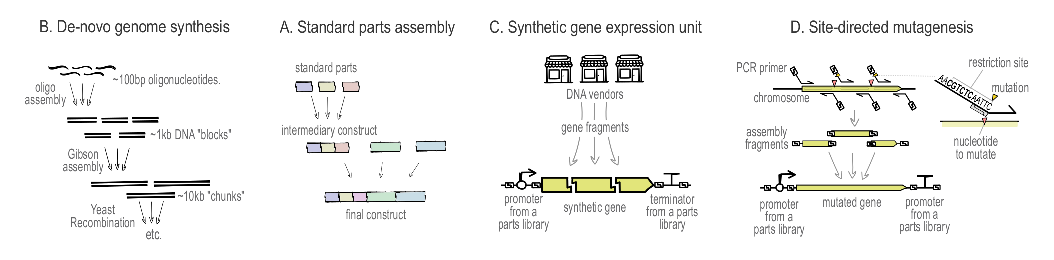
\includegraphics[width=\textwidth]{figures/figure_1_dna_projects.eps}
  \caption{Illustration of different categories of DNA construction projects. The schemas focus on the assembled parts and do not show the plasmid backbones necessary for assembly selection and amplification. \textbf{(A)} First steps of the hierarchical assembly of an artificial chromosome in the Sc2.0 project.
\textbf{(B)} 2-step assembly of standard genetic parts. The second step can use a mix of intermediary constructs and standard genetic parts.
\textbf{(C)} Golden Gate Assembly of a gene expression unit using standard promoter and terminator parts from a library, and a long synthetic gene bought in three fragments from commercial vendors, resulting in a five-part assembly.
\textbf{D} Assembly of a gene expression unit using standard promoter and terminator parts, as in Panel C, but where the gene obtained from the chromosome of an organism via PCR. Red triangles on the chromosome indicate the position of BsmBI sites which preclude Golden Gate assembly, and are mutated away in the final sequence.}
  \label{dna_projects}
\end{figure}


\begin{figure}[!tpb]
  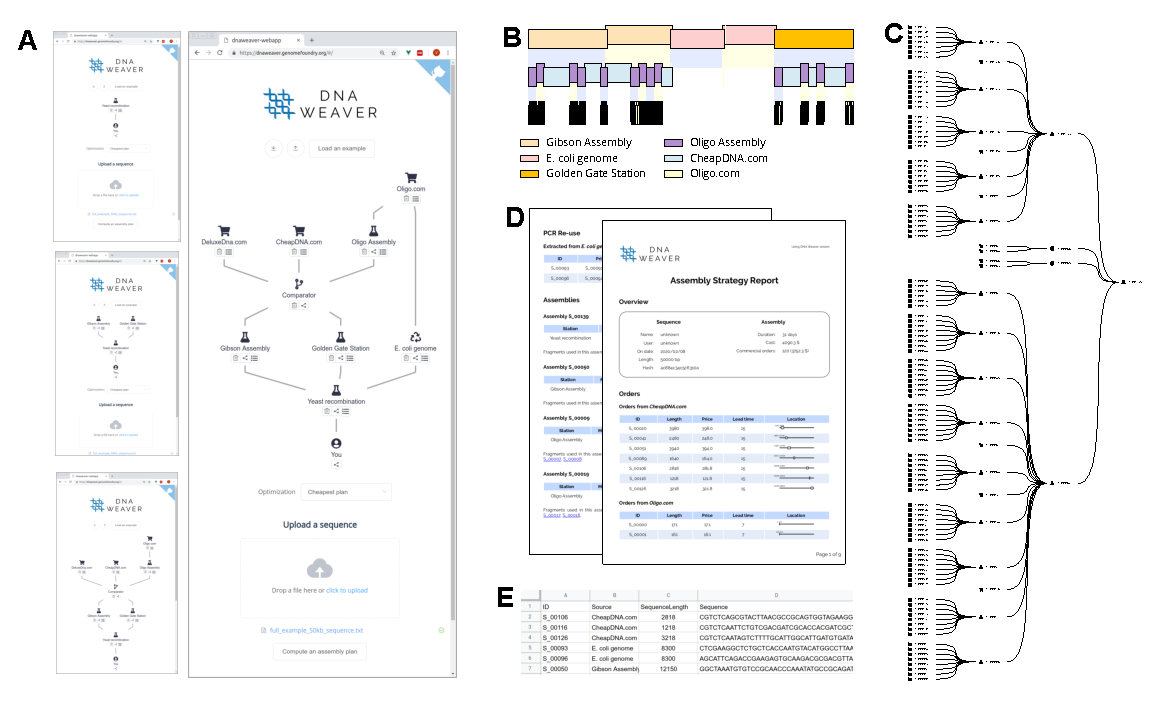
\includegraphics[width=\textwidth]{figures/figure_2_app_screenshots.eps}
  \caption{The DNA Weaver web application and its output. The scenario described in this figure can be loaded and experimented with via the "Load an example" button of the web application.
\textbf{(A)} DNA supply network defined via the web interface. Miniatures on the left show the chronological order of the network's construction. Small icons under a station lead to menus to select parameters and suppliers.
\textbf{(B)} Schema of the multi-step construction plan (from bottom to top) of a 50kb sequence, devised by the web application with respect to the supply network in Panel A, in under 10 seconds. Each rectangle represents a DNA fragment whose color indicates the provenance. The top line shows the fragments of the final assembly: the plan takes advantage of a large homology of the sequence with \textit{E. coli} to obtain the central part via PCR. The second line shows the origin of the blocks used in Gibson Assembly or Golden Gate assembly. In this plan, the fragments come either from CheapDNA or the assembly of oligonucleotides (represented on the third line). This schema is appears as a PDF file in the multi-file report generated by DNA Weaver.
\textbf{(C)} Summary PDF report indicating the different assembly steps and listing all assembly fragments ordered or built.
\textbf{D} Spreadsheet listing the sequence of every fragment or primer to order, and every assembled fragment.
\textbf{E} Map of the assembly plan providing an alternative view to the Panel B schema, with the identifiers of the different fragments and primers involved in the assembly.}
  \label{app_screenshots}
\end{figure}



\begin{figure}[!tpb]
  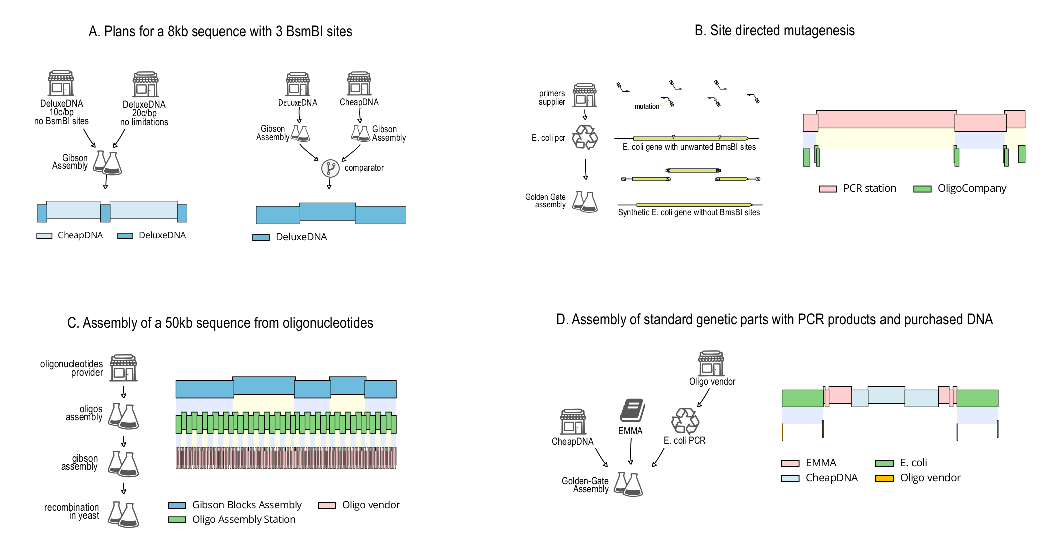
\includegraphics[width=\textwidth]{figures/figure_3_example_supply_networks.eps}
  \caption{
Examples of DNA Weaver supply networks for different DNA Construction problems. The assembly plan summary plots in each panel can be generated using the examples provided in the DNA Weaver Github repository. Each rectangle represents an assembly fragment or primer, and colors indicate each fragment's origin (see the caption of Figure 2B for details).
\textbf{(A)} Multi-vendor problem. A 10kb DNA sequence containing 3 BsmBI restriction sites will be assembled via Gibson assembly using fragments comming from one of two vendors: CheapDNA charges 10c per basepair but won't synthesize fragments containing a BsmBI site. DeluxeDNA can produce any fragment for 20c/bp. Both stations only sell fragments under 4kb. In the left network, each fragment can be ordered from a different vendor, resulting in a plan using CheapDNA as much as possible, and DeluxeDNA only in regions harboring a BsmBI site. The right-hand network compares two assembly workflows where all DNA fragments come from a single source. As a result, the assembly plan suggested catters to the cheapest provider able to provide all fragments at once.
\textbf{B} Site directed mutagenesis, as presented in Figure 1C. This problem can be modelled as a linear supply network comprising a commercial primers vendor, an \textit{E. coli} PCR station, and a Golden Gate Assembly station. The sequence to assemble, a synthetic \textit{E. coli} gene edited to remove BsmBI sites, will be created by ordering primers from the vendor, using them in the PCR station to amplify the chromosome fragments to be assembled.
\text{C} Hierarichical assembly of an arbitrary sequence from oligonucleotides. This example mimics the protocol of Figure 1A with a linear supply network chaining different assembly stations which feed each other with increasingly large DNA fragments.
\text{D} Supply network for the assembly of a gene expression unit from various sources. The sequence to build contained a coding sequence that must be ordered commercially, flanked by 6 standard parts from the EMMA Assembly standard, and 2 homology harms for integration in \textit{E. coli}. The assembly plan correctly detected that the reusable EMMA parts and homologies.}
  \label{app_screenshots}
\end{figure}


\begin{figure}[!tpb]
  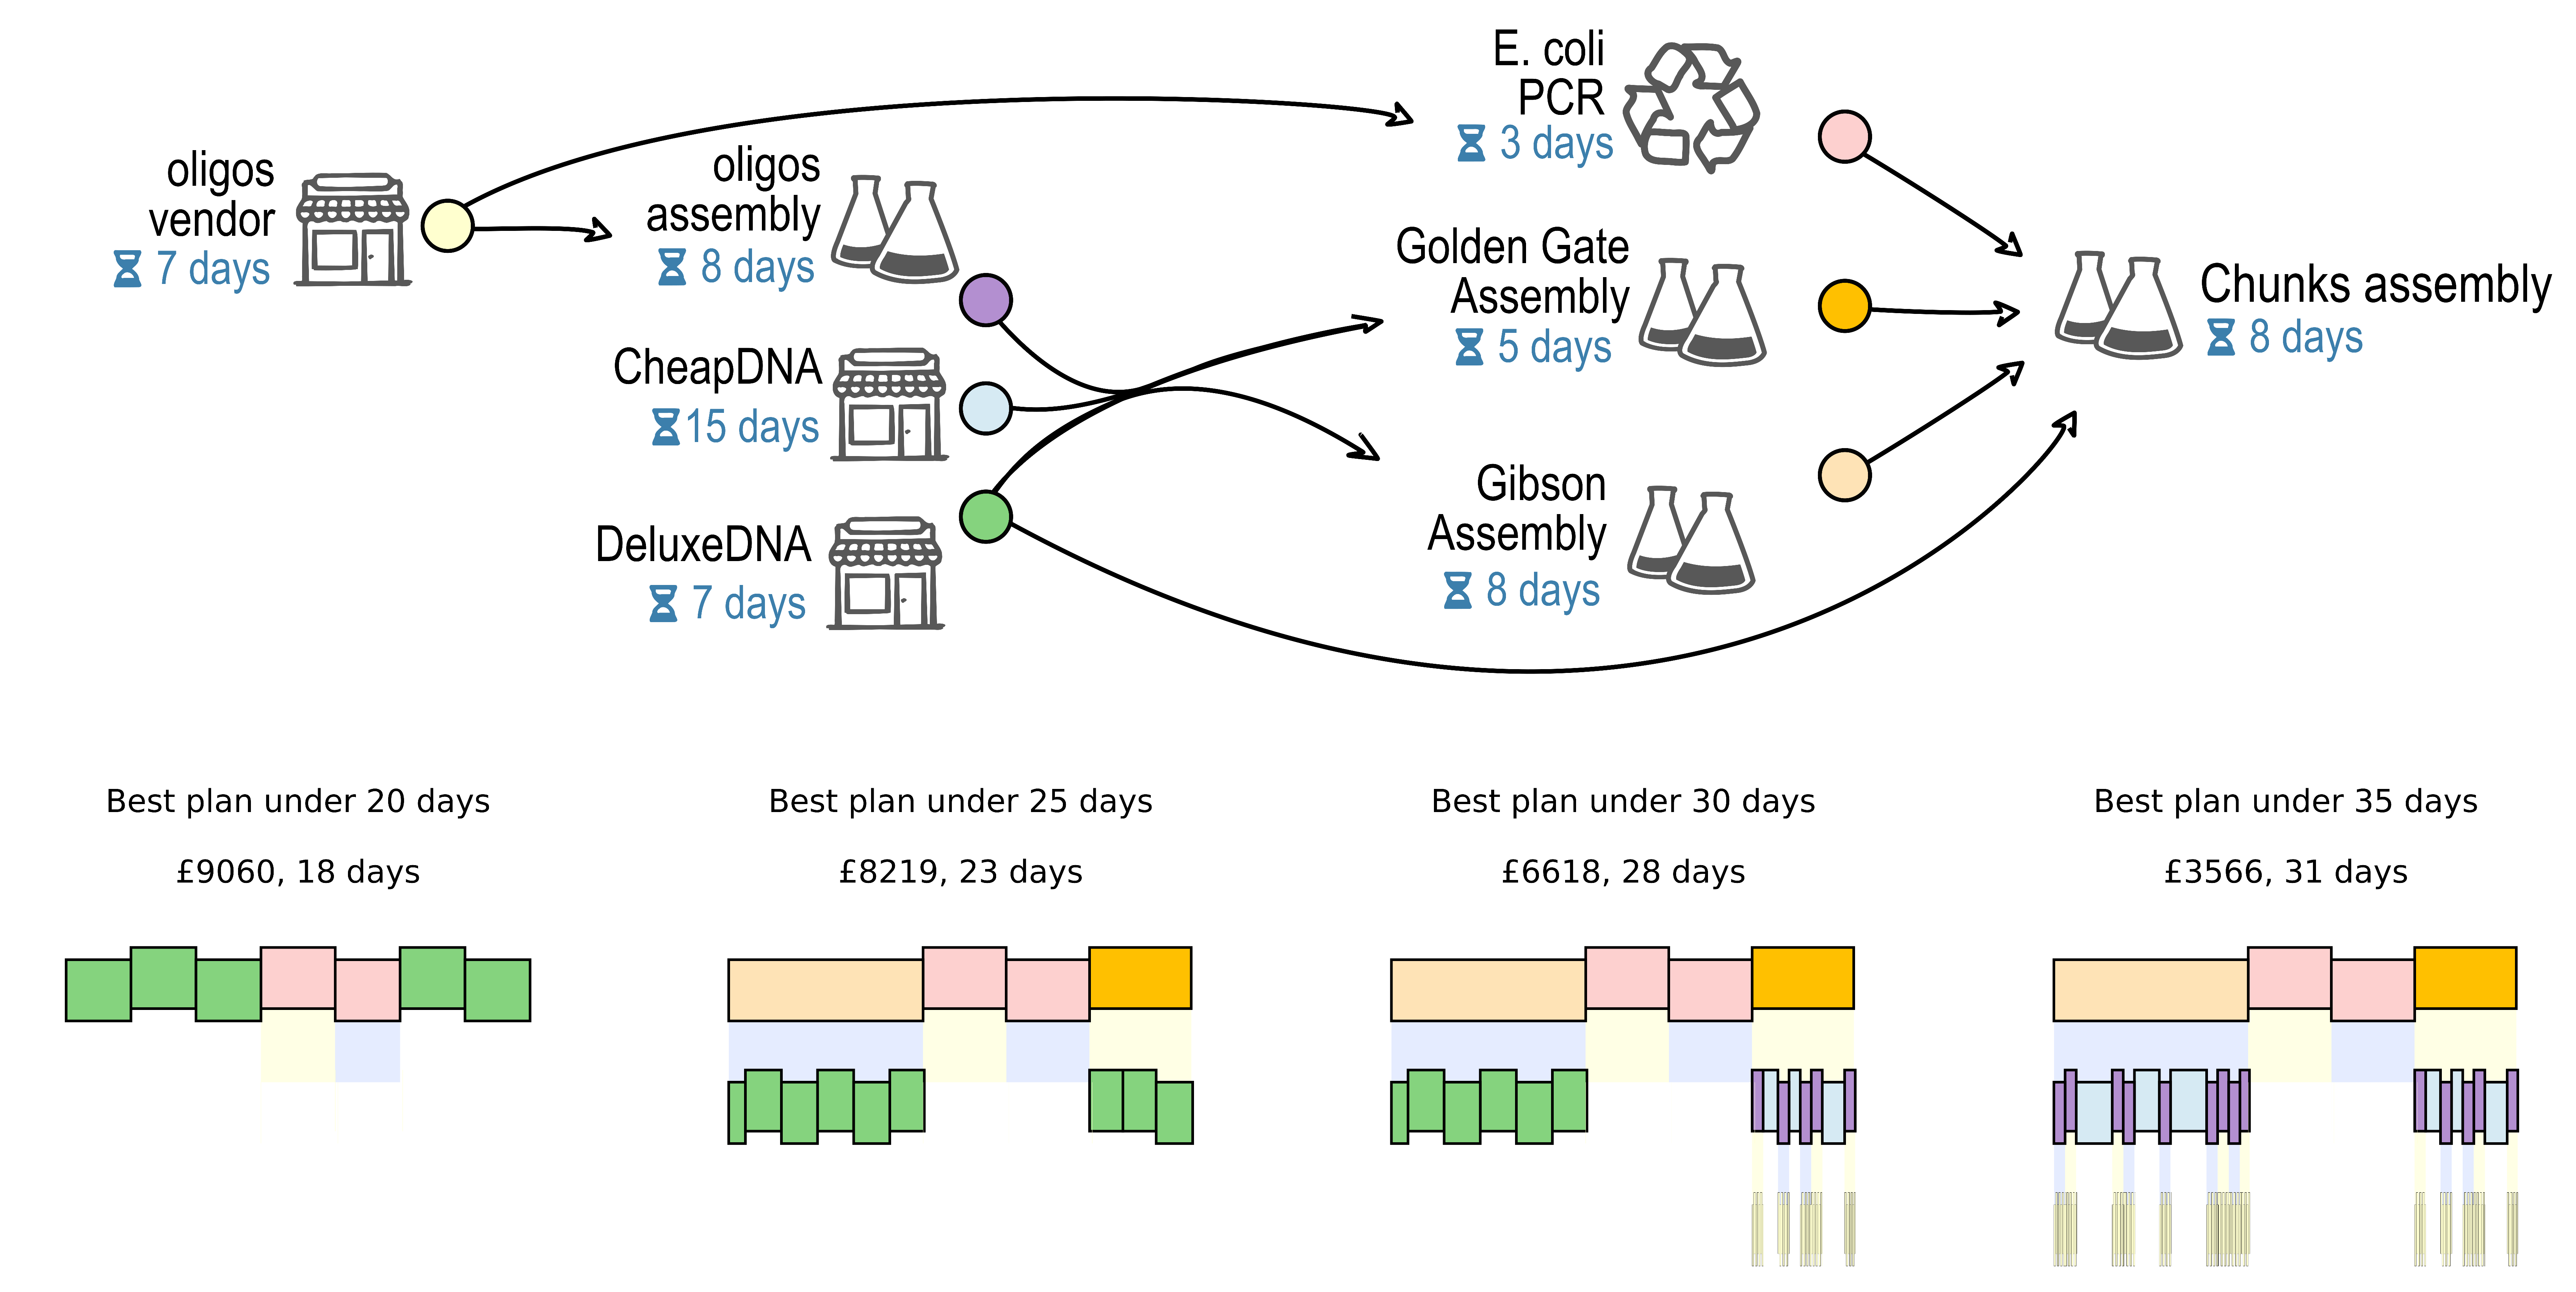
\includegraphics[width=\textwidth]{figures/figure_4_time_limit.eps}
  \caption{Effect of lead time constraints on the assembly plan returned by DNA Weaver. The supply network is a variant of the network described in Figure 1, where the typical lead time of each station, in days, is specified. The assembly plots below show four plans computed for the sequence of Figure 1, but for increasing large maximal lead times used as parameters.} 
  \label{lead_time}
\end{figure}


\begin{figure}[!tpb]
  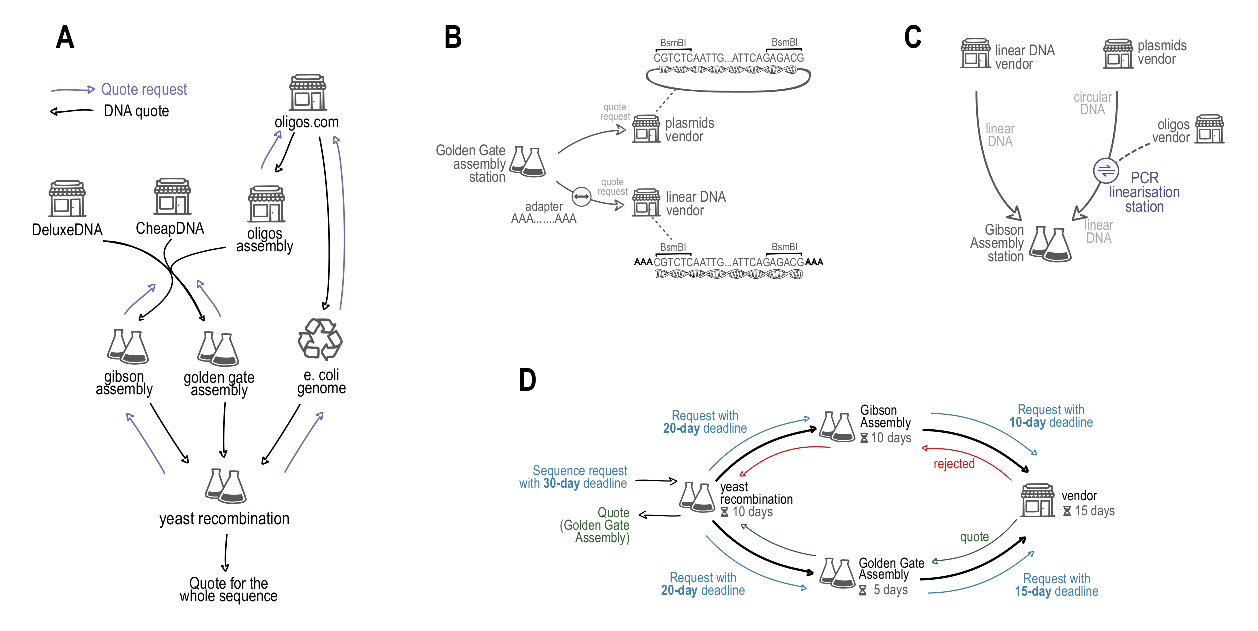
\includegraphics[width=\textwidth]{figures/figure_5_supply_networks_function.eps}
  \caption{Exchanges between the stations of a supply network.
  \textbf{(A)} Direction of requests and sequence quotes in the supply network of Figure 2A.
  \textbf{(B)} Supply network where a same sequence, flanked by cloning restriction sites, can be requested to two different suppliers producing respectively linear and circular DNA. A sequence extension station is intercaled before the linear DNA vendor to add a few basepairs to the sequence flanks and avoid having the restriction sites at the end of the sequence.
  \textbf{C} Two vendors, offering respectively linear and circular DNA, supply fragments for a Gibson Assembly. A PCR linearization station and a primers supplier are added before the circular DNA vendor, to take into account the linearization of fragments required by Gibson Assembly.
  \textbf{D} Example of requests and responses between the elements of a network in presence of a maximal lead time constraint. Here it is assumed that the researcher modeled Gibson Assembly as twice longer to perform than Golden Gate assembly. As a result, the chain of requests going through the Gibson Assembly station yields only refusals from the DNA vendor, due to too short delays, and the assembly plan returned by the solver will use Golden Gate assembly.}
  \label{supply_networks}
\end{figure}


\begin{figure}[!tpb]
  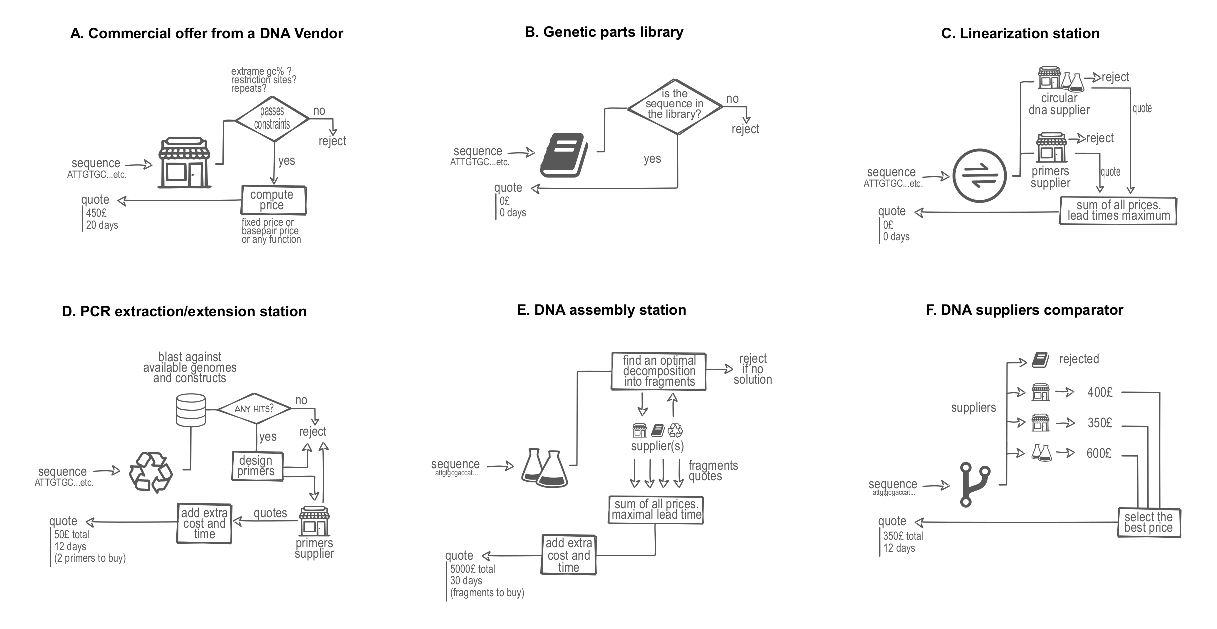
\includegraphics[width=\textwidth]{figures/figure_6_supply_network_elements.eps}
  \caption{Internal mechanisms of built-in DNA supplier classes}
  \label{dna suppliers_internals}
\end{figure}


\begin{figure}[!tpb]
  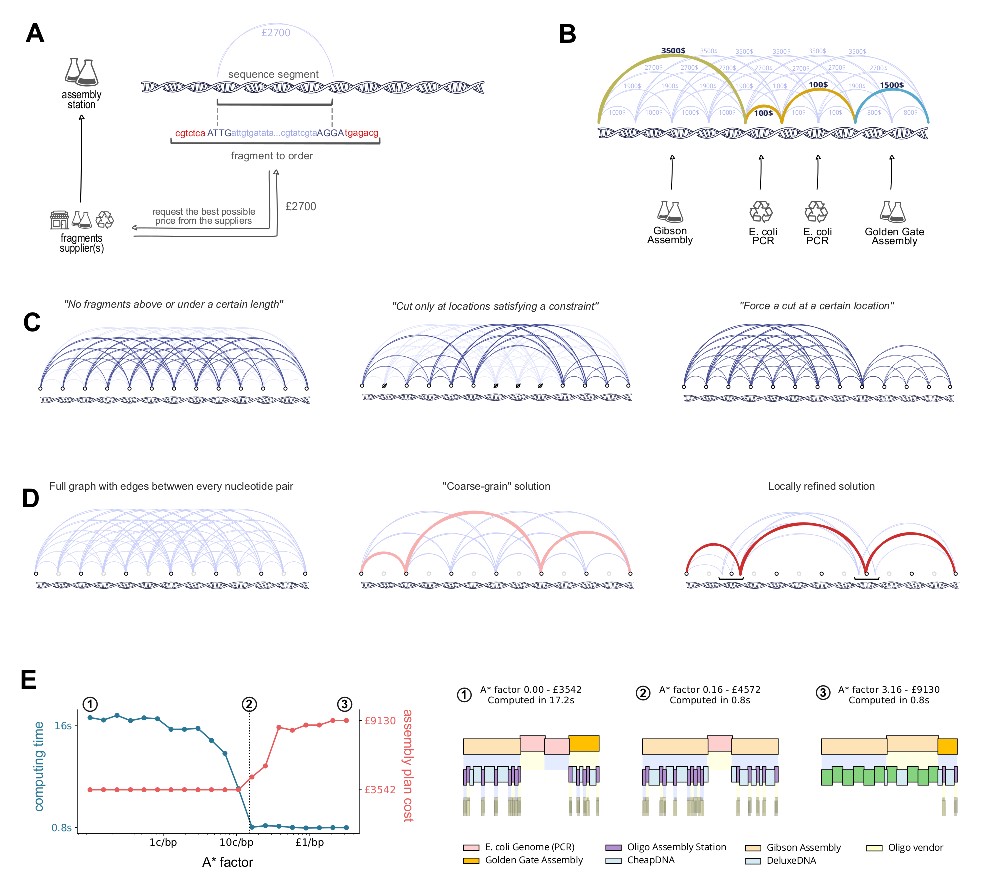
\includegraphics[width=\textwidth]{figures/figure_7_graph_algorithms.eps}
  \caption{Graph-based sequence decomposition methods.}
  \label{dna suppliers_internals}
\end{figure}

\begin{figure}[!tpb]
  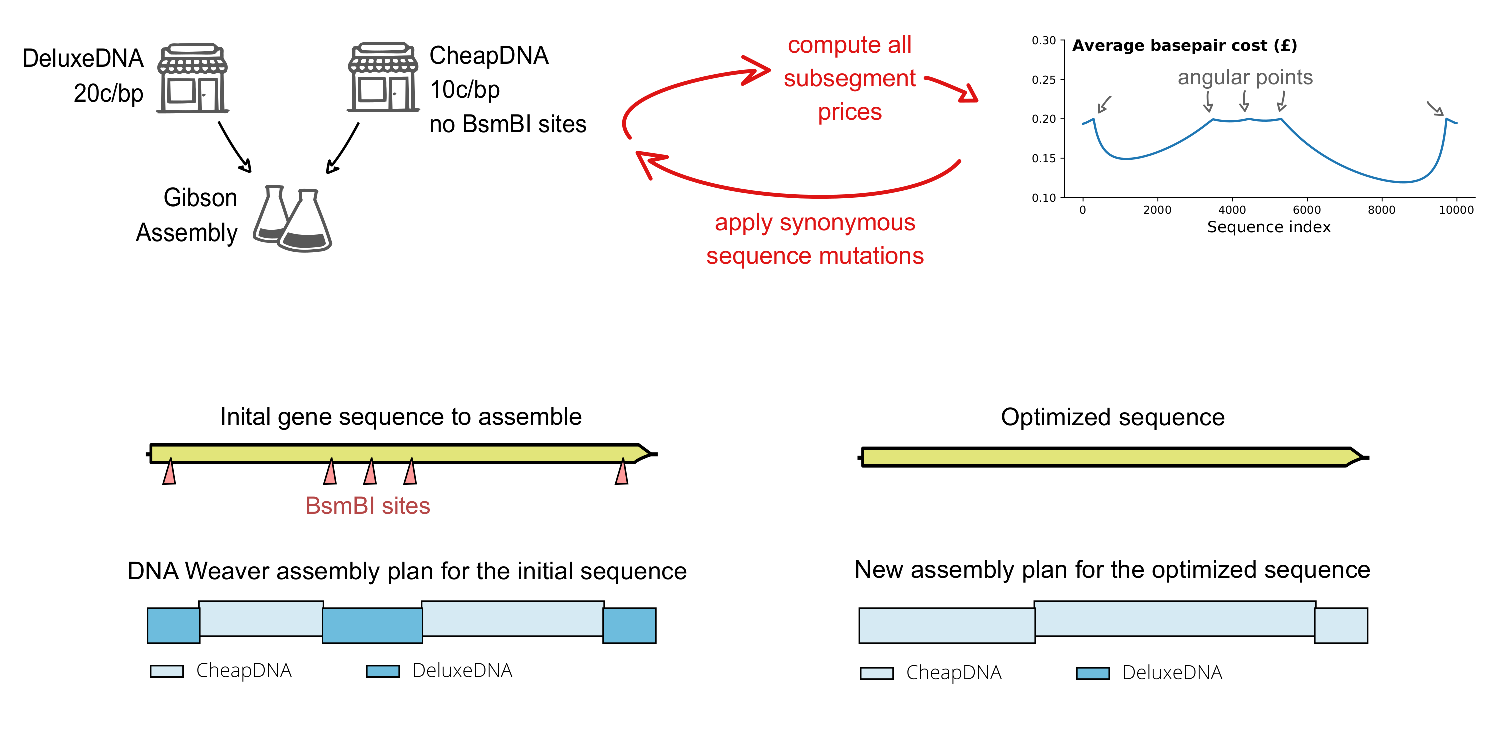
\includegraphics[width=\textwidth]{figures/figure_8_manufacturability-optimization.eps}
  \caption{Internal mechanisms of built-in DNA supplier classes}
  \label{dna suppliers_internals}
\end{figure}
\end{document}